%# -*- coding:utf-8 -*-
\documentclass[fontset=windows]{article}
\usepackage[final]{neurips_2022}

\usepackage[UTF8]{ctex}
\usepackage[numbers, sort&compress]{natbib}
\usepackage[T1]{fontenc}    % use 8-bit T1 fonts
\usepackage{hyperref}       % hyperlinks
\usepackage{url}            % simple URL typesetting
\usepackage{booktabs}       % professional-quality tables
\usepackage{amsfonts}       % blackboard math symbols
\usepackage{nicefrac}       % compact symbols for 1/2, etc.
\usepackage{microtype}      % microtypography
\usepackage{xcolor}         % colors
\usepackage{graphicx}       % 图片包
\usepackage{subfig}
\usepackage{geometry}
\usepackage{calligra}
\usepackage{algorithm}
\usepackage{algorithmicx}
\usepackage{algpseudocode} 
\usepackage{amsmath}
\usepackage{amssymb}
\usepackage{bm}
\usepackage{multirow}
\usepackage{diagbox}
\usepackage{tablefootnote}
\usepackage{indentfirst}
\usepackage{amssymb}
\setlength{\parindent}{2em}
\newtheorem{definition}{Definition}[section]
\newtheorem{theorem}{Theorem}[section]
\newtheorem{notations}{Notations}

% \hypersetup{
%   colorlinks=true,
%   linkcolor=cyan,
%   filecolor=red,      
%   urlcolor=blue,
%   citecolor=green,
% }
\title{基于CIE 1931-XYZ与CIE 2006-XYZ色彩空间的光源光谱和色域特性计算}

\author{%
    刘昭炀\\ %\thanks{Use footnote for providing further information
    电子与信息工程学院\quad 信息与通信工程\\
    22215608\\
    \href{mailto:liuzhy86@mail2.sysu.edu.cn}{liuzhy86@mail2.sysu.edu.cn}\\
}

\begin{document}

\maketitle

\begin{abstract}
    \qquad 色彩是一种人类大脑的主观感受,不同人所感知的颜色也会有所区别。色彩是一个心理量,人们使用RGB模型将其公理化。根据混色原理,RGB模型可表征所有色彩,但由于RGB模型的三刺激值之一r存在负值使用不方便,因此对RGB系统进行线性变化,得到没有负值的XYZ系统。本文将基于$2^\circ$观察视角的CIE 1931-XYZ与CIE 2006-XYZ色彩空间,对LED数据\footnote{数据来源:\url{https://sites.psu.edu/llab/downloads/}}做光源光谱和色域特性计算。

    \qquad 本文使用Python\footnote{本文源代码可见于:\url{https://github.com/AnnLIU15/modern-optics-hw}}基本实现了``光源光谱与色域特性计算''题目的四个子目标:光谱图、色品图与最大色域四基色(ABCD),部分借鉴了开源项目Colour\footnote{Colour:\url{https://www.colour-science.org/}}的思路并按自己的理解实现对应其功能。
\end{abstract}

% footnote ref: https://arxiv.org/pdf/2108.10026.pdf
\begingroup
\let\clearpage\relax
\section{引言}

环境中的可见光(380nm$\sim$780nm)可被人视网膜上的锥状细胞感知,然后经过视觉系统传输、处理至大脑,大脑会``想象''出来这些光所组成的色彩。简而言之,感光是一种客观规律,而色彩便是一种主观感受。

人的视网膜上有四种感知光的细胞,包括了三种锥状细胞与一种杆状细胞,三种锥状细胞分别感知红(Red,R),绿(Green,G),蓝(Blue,B)三色,杆状细胞感知黑白(亮度)。三种锥状细胞感知最灵敏的称为三原色,但是这三种颜色并不满足Grassmann的混色原理/视觉三基色假说\cite{grassmann1853theorie},不能混出所有可见光范围内的所有颜色。基于人眼三原色与混色原理,国际照明委员会(Commission Internationale de l´Eclairage,CIE)在1931年制定了三基色的统一标准,将700nm、546.1nm、435.8nm的单色光视为红、绿、蓝三原色,也被称为物理三基色,所有可见光都可由三种颜色混合而来。

\subsection{RGB色彩空间}

\begin{figure}[htbp]
    \centering
    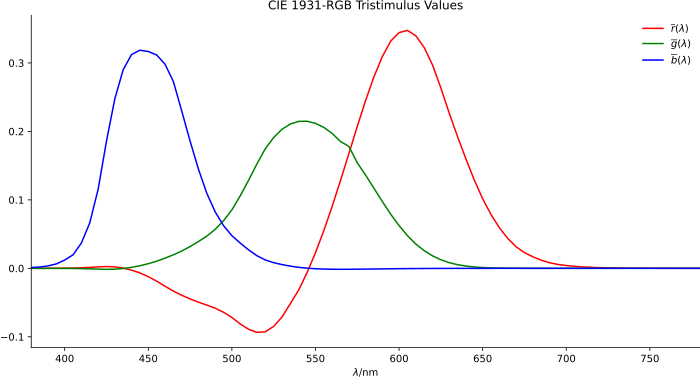
\includegraphics[width=0.8\textwidth]{./imgs/sec1/rgb-1931.pdf}
    \caption{CIE 1931-RGB色彩空间色彩匹配函数}
    \label{fig:tri-rgb}
 \end{figure}

从上文我们得知了RGB三基色,CIE在提出RGB系统的同时,通过实验确定确定了各个单波长的三刺激值,得到了色彩匹配函数(Color matching function,CMF),如图\ref{fig:tri-rgb}所示。色彩匹配函数是视觉系统的固有属性,是一个客观存在的量。我们只需将光谱数据与色彩匹配函数做一个积分、求和\eqref{eq:tri-rgb},便可以获取其RGB相关信息。通过对RGB进行归一化\eqref{eq:tri-rgb-n},便可以获取到色品坐标$(r,g)$,就能唯一确定一种颜色。

\begin{equation}
    \begin{aligned}
        R & =\int \overline{r}(\lambda)\cdot\psi(\lambda)\text{d}\lambda \quad\text{or}\quad R = \sum_{380\text{nm}}^{780\text{nm}} \overline{r}(\lambda)\cdot\psi(\lambda)\\
        G & =\int \overline{g}(\lambda)\cdot\psi(\lambda)\text{d}\lambda \quad\text{or}\quad G = \sum_{380\text{nm}}^{780\text{nm}} \overline{g}(\lambda)\cdot\psi(\lambda)\\
        B & =\int \overline{b}(\lambda)\cdot\psi(\lambda)\text{d}\lambda \quad\text{or}\quad B = \sum_{380\text{nm}}^{780\text{nm}} \overline{b}(\lambda)\cdot\psi(\lambda)\\
    \end{aligned}
    \label{eq:tri-rgb}
\end{equation}

\begin{equation}
    \begin{aligned}
        r & =\frac{R}{R+G+B}\\
        g & =\frac{G}{R+G+B}\\
        b & =\frac{B}{R+G+B} = 1-r-g\\
    \end{aligned}
    \label{eq:tri-rgb-n}
\end{equation}

但是从图\ref{fig:tri-rgb}中可以看出CIE 1931-RGB色彩空间色彩匹配函数中$r$存在负值,不方便计算以及不符合人类的直观感受,并且由于负值的存在,从$C=R+G+B$的三刺激值中无法直观地理解。为了消除这部分负值的影响以及均匀度的问题,CIE组织提出了几种由RGB空间线性、非线性变换得来的色彩空间,如XYZ、Lab、Luv。本文基于的题目便是当中的一种线性变换色彩空间--XYZ。

\subsection{XYZ色彩空间}

\begin{figure}[htbp]
    \centering
    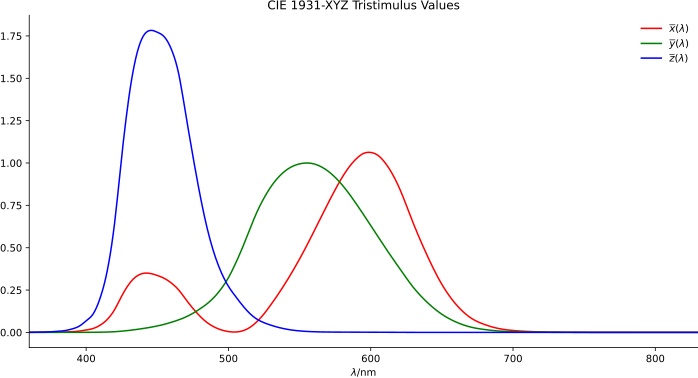
\includegraphics[width=0.8\textwidth]{./imgs/sec1/xyz-1931.pdf}
    \caption{CIE 1931-XYZ色彩空间色彩匹配函数}
    \label{fig:tri-xyz}
 \end{figure}

在CIE 1931-XYZ色彩空间空间中,虚构了X(红)、Y(绿)、Z(蓝)三原色,同时解决了亮度叠加($C=X+Y+Z$)与色彩匹配函数负值问题,色彩匹配函数如图\ref{fig:tri-xyz}所示。与RGB色彩空间一样,我们只需将光谱数据与色彩匹配函数做一个积分、求和\eqref{eq:tri-xyz},便可以获取其XYZ相关信息,其中$Y$为色光的亮度,$k$根据亮度$Y$的需求决定。通过对XYZ进行归一化\eqref{eq:tri-xyz-n},便可以获取到色品坐标$(x,y)$,也能唯一确定一种颜色。XYZ色彩空间三刺激值与RGB色彩空间三刺激值的线性转换如公式\eqref{eq:tri-xyz-rgb}所示。

\begin{equation}
    \begin{aligned}
        X & =k\int \overline{x}(\lambda)\cdot\psi(\lambda)\text{d}\lambda \quad\text{or}\quad R = k\sum_{380\text{nm}}^{780\text{nm}} \overline{x}(\lambda)\cdot\psi(\lambda)\\
        Y & =k\int \overline{y}(\lambda)\cdot\psi(\lambda)\text{d}\lambda \quad\text{or}\quad G = k\sum_{380\text{nm}}^{780\text{nm}} \overline{y}(\lambda)\cdot\psi(\lambda)\\
        Z & =k\int \overline{z}(\lambda)\cdot\psi(\lambda)\text{d}\lambda \quad\text{or}\quad B = k\sum_{380\text{nm}}^{780\text{nm}} \overline{z}(\lambda)\cdot\psi(\lambda)\\
        k & = \frac{1}{Y} (\frac{100}{Y},\frac{683}{Y})\\
    \end{aligned}
    \label{eq:tri-xyz}
\end{equation}

\begin{equation}
    \begin{aligned}
        x & =\frac{X}{X+Y+X}\\
        y & =\frac{Y}{X+Y+X}\\
        z & =\frac{Z}{X+Y+X} = 1-x-y\\
    \end{aligned}
    \label{eq:tri-xyz-n}
\end{equation}

\begin{equation}
    \begin{bmatrix}
        \overline{r}\\
        \overline{g}\\
        \overline{b}\\
    \end{bmatrix} = \begin{bmatrix}
    0.41846 & -0.15860 & -0.08283\\
    -0.09117 & 0.25243 & 0.01571\\
    0.00092 & -0.00255 & 0.17860\\
    \end{bmatrix}\begin{bmatrix}
        \overline{x}\\
        \overline{y}\\
        \overline{z}\\
    \end{bmatrix}
    \label{eq:tri-xyz-rgb}
\end{equation}


从上一小节我们曾提到,XYZ是RGB经转化而来的,由于本人的仿真所在的操作系统的是Windows,缺省的色彩模式为Standard RGB(sRGB),因此我们将此处的RGB默认为sRGB,XYZ转sRGB还需要一段非线性函数进行校正(gamma校正),sRGB转XYZ(Y=1)如公式\eqref{eq:trans-srgb2xyz}所示,XYZ(Y=1)转sRGB如公式\eqref{eq:trans-xyz2srgb}所示。

\begin{equation}
    \begin{aligned}
        \begin{bmatrix}
            sR^\prime\\
            sG^\prime\\
            sB^\prime\\
        \end{bmatrix} & = V^\prime = \left\{ \begin{matrix}
            \frac{V}{12.92} & V\leq 0.04045 \\
            (\frac{V+0.055}{1.055})^{2.4} & V> 0.04045 \\
        \end{matrix} \right.
        \\
        \begin{bmatrix}
            X\\
            Y\\
            Z\\
        \end{bmatrix} &= 
        \begin{bmatrix}
            0.4124 & 0.3576 & 0.1805\\
            0.2126 & 0.7152 & 0.0722\\
            0.0193 & 0.1192 & 0.9505\\
        \end{bmatrix}\begin{bmatrix}
            sR^\prime\
            sG^\prime\
            sB^\prime\
        \end{bmatrix} 
    \end{aligned}
    \label{eq:trans-srgb2xyz}
\end{equation}

\begin{equation}
    \begin{aligned}
        C_\text{linear} = \begin{bmatrix}
            R^\prime\\
            G^\prime\\
            B^\prime\\
        \end{bmatrix} &= 
        \begin{bmatrix}
            3.24062548& -1.53720797 & -0.49862860\\
            -0.96893071& 1.87575606 & 0.04151752\\
            0.05571012& -0.20402105 & 1.05699594\\
        \end{bmatrix}\begin{bmatrix}
            X\\
            Y\\
            Z\\
        \end{bmatrix} \\
        \begin{bmatrix}
            R\\
            G\\
            B\\
        \end{bmatrix} &= \left\{ \begin{matrix}
            \max(12.92\cdot C_\text{linear},0) & C_\text{linear}\leq 0.0031308 \\
            1.055(C_\text{linear}^\frac{1}{2.4}) - 0.055 & C_\text{linear}> 0.0031308 \\
        \end{matrix} \right.
    \end{aligned}
    \label{eq:trans-xyz2srgb}
\end{equation}

从公式中我们可以知道,理论上存在颜色相同而光谱不同的非纯色光,混色的方法有很多种。

CIE 1931-XYZ的色彩也是基于人测定的,由于一些较纯的色彩在实际中并不会用到以及新的实验,CIE提出了CIE 2006-XYZ色彩空间,其对xyz三刺激值做了一些修正(主要为蓝色),如图\ref{fig:tri-xyz-2}所示。从图中我们可以知道,除蓝色的峰值外,CIE 2006-XYZ色彩相较于CIE 1931-XYZ区别不大。

\begin{figure}[htbp]
    \centering
    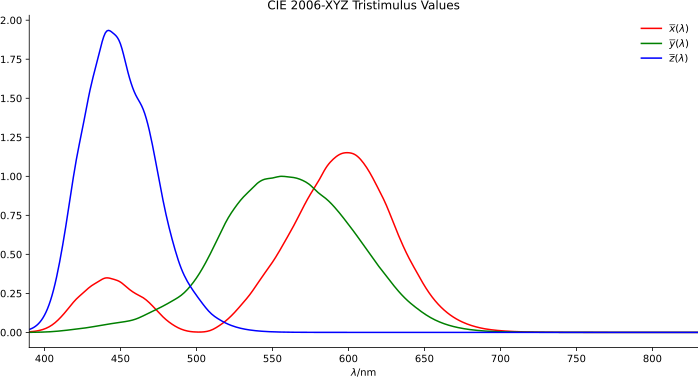
\includegraphics[width=0.8\textwidth]{./imgs/sec1/xyz-2006.pdf}
    \caption{CIE 2006-XYZ色彩空间色彩匹配函数}
    \label{fig:tri-xyz-2}
 \end{figure}  % 引言
\section{光谱功率分布}
题目中第一个任务为将给定光谱转换为光谱功率分布图,并以可见光的光谱作为背景板。首先我们实现可见光谱背景,将波长转换为sRGB颜色。

\subsection{可见光谱的sRGB颜色}

首先我们知道XYZ空间是可以转换为RGB空间的,并且由于后面需要画XYZ空间的色品图,因此本文的可见光谱的绘制也是由xyz空间出发,将单色光的xyz数据转化为sRGB数据,并作出可见光谱背景。

那么我们首先需要根据波长计算出对应的单色光颜色。我们先考虑一个问题,XYZ中的绝对大小有意义吗?从公式\eqref{eq:tri-xyz}与公式\eqref{eq:tri-xyz-n}来看,XYZ在计算的时候会根据Y大小进行缩放,并且xyz与xyY(不计算z,认为Y=1)并不关心XYZ原本积分与求和得到的绝对值,因此我们可以认为,归一化的光谱是不会影响色品图中xy坐标的,故也不会改变颜色。所以我们可以认为,单色光仅在380$\sim$780nm的波段上的某个波长上有非零值,且改非零值为1(后续我们将以求和公式计算XYZ,积分时候为一个冲激函数),后续将$XYZ$进行放缩,令$Y=1$,如公式\eqref{eq:wavelength2xyz}所示。

\begin{equation}
    \begin{aligned}
        X(\lambda^\prime) & =k\sum_{380\text{nm}}^{780\text{nm}} \overline{x}(\lambda)\cdot\psi(\lambda) = k \overline{x}(\lambda) = \frac{\overline{x}(\lambda)}{\overline{y}(\lambda)}\\
        Y(\lambda^\prime) & =k\sum_{380\text{nm}}^{780\text{nm}} \overline{y}(\lambda)\cdot\psi(\lambda) = k \overline{y}(\lambda) = 1\\
        Z(\lambda^\prime) & =k\sum_{380\text{nm}}^{780\text{nm}} \overline{z}(\lambda)\cdot\psi(\lambda) = k \overline{z}(\lambda) = \frac{\overline{Z}(\lambda)}{\overline{y}(\lambda)}\\
        k & = \frac{1}{Y(\lambda^\prime)}\\
    \end{aligned}
    \label{eq:wavelength2xyz}
\end{equation}

在Colour中,会先对三刺激值进行色度自适应变换(Chromatic adaptation matrix),使用CAT02矩阵\eqref{eq:CAT02}将XYZ值线性变换到LMS空间,然后将以CIE标准白光D65作为参考点的XYZ转化为等能白光E为参考点的XYZ,然后再乘上CAT02矩阵的逆矩阵回到XYZ空间,做一个白光的自适应处理,本文也做了此步,但发现与没做并无明显区别,其完整过程如公式\eqref{eq:CAT}所示,其中三刺激值的维度为$(401,3)$。

\begin{equation}
    M_{CAT02} = \begin{bmatrix}
        0.7328  & 0.4296 & -0.1624\\
        -0.7036 & 1.6975 & 0.0061\\
        0.0030  & 0.0136 & 0.9834\\
    \end{bmatrix}
    \label{eq:CAT02}
\end{equation}

\begin{equation}
    \begin{bmatrix}
        \overline{x^\prime}\\
        \overline{y^\prime}\\
        \overline{z^\prime}\\
    \end{bmatrix} = \begin{bmatrix}
        \overline{x}\\
        \overline{y}\\
        \overline{z}\\
    \end{bmatrix}\cdot ((M_{CAT02})^{-1}\cdot D_\frac{E}{D65}\cdot M_{CAT02})^T = \begin{bmatrix}
        \overline{x}\\
        \overline{y}\\
        \overline{z}\\
    \end{bmatrix} \cdot \begin{bmatrix}
        0.96621  & -0.04045 & 0.02469\\
       -0.02868  &  1.01863 & 0.01005\\
        0.00077  &  0.00107 & 1.08721\\
    \end{bmatrix}^T
    \label{eq:CAT}
\end{equation}

由上式可见,变换矩阵和方阵的区别不大,变换细微,因此不放没有处理的图,依据上述流程先对三刺激值进行白光D65到白光E的自适应\eqref{eq:CAT},然后求得XYZ值\eqref{eq:CAT02},最后使用变换公式将单色光的XYZ转化为sRGB\eqref{eq:trans-xyz2srgb},结果如图\ref{fig:wave}所示,由于pdf等格式有很明显的柱状图显示问题,因此光谱分布这一部分使用300dpi的png格式文件。

\begin{figure}[htbp]
    \centering
    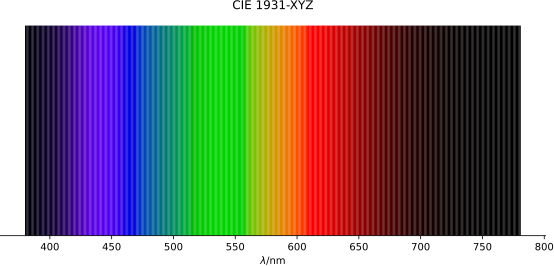
\includegraphics[width=0.65\textwidth]{"./imgs/sec2/CIE 1931-XYZ-spd.png"}
    \caption{CIE 1931-XYZ可见光谱}
    \label{fig:wave}
\end{figure}


\subsection{光谱功率分布图与分析}

\begin{figure}[htbp]
    \centering
    \includegraphics[width=0.65\textwidth]{"./imgs/sec2/CQS-1-NM-spd-rgb.pdf"}
    \caption{基于CIE 1931-XYZ的光谱功率分布图 -- 无背景}
    \label{fig:spd1931nobg}
\end{figure}

解决了可见光谱的问题,接下来就十分简单了,只需要录入数据,设定好波长范围与归一化的预处理(全局或者每通道归一化),画到图上即可。

本文的LED数据来源为宾夕法尼亚州立大学照明实验室(llab),具体网址可见首页脚注,本文将RGB三色数据提取出来,匹配CIE格式(txt,csv)。最终的谱功率分布图如图\ref{fig:spd1931nobg}(无背景)、图\ref{fig:spd1931bg}(未通道归一化)与图\ref{fig:spd1931bgn}(通道归一化)所示。大体操作可见于\textbf{utils/get\_spd.py}中的\textit{get\_spd}函数与\textit{spd\_background}函数。



\begin{figure}[htbp]
    \centering
    \includegraphics[width=0.65\textwidth]{"./imgs/sec2/CQS-1-NM-1931-spd.png"}
    \caption{基于CIE 1931-XYZ的光谱功率分布图}
    \label{fig:spd1931bg}
\end{figure}

\begin{figure}[htbp]
    \centering
    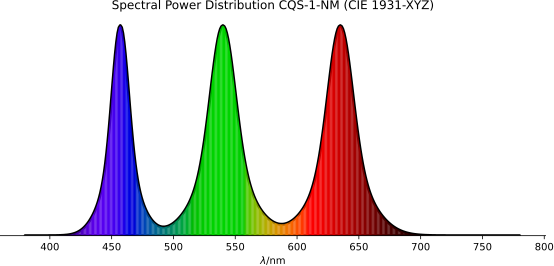
\includegraphics[width=0.65\textwidth]{"./imgs/sec2/CQS-1-NM-1931-spd-n.png"}
    \caption{基于CIE 1931-XYZ的光谱功率分布图 -- 通道归一化}
    \label{fig:spd1931bgn}
\end{figure}

如上所示,我们完成了第一个子目标,完成了光谱图的绘制。  % 定义
\section{CIE 1931-XYZ空间}
题目中第二个任务为画出色品图,并在其上面画出LED RGB三色灯所组成的色域维度,并与NTSC色域进行对比,给出百分比定量结论。首先我们实现色品图,其原理与上一节的一样,将波长单色光转化为范围约束线,坐标转换为sRGB颜色,基本流程与上一节大同小异。

\subsection{CIE 1931-XYZ空间 -- 色品图}

色品图的绘制关键在于限定马蹄的边缘以及图上的每一点,从上一节我们得知可见光XYZ值是如何得来的\eqref{eq:wavelength2xyz}。因此我们得到了每个波长的XYZ,根据公式\eqref{eq:tri-xyz-n}我们便可以得到每个波长在色品图中的坐标点。如图\ref{fig:sd1931edges}所示。

\begin{figure}[htbp]
    \centering
    \includegraphics[width=0.65\textwidth]{./imgs/sec3/cd-edge-s.pdf}
    \caption{基于CIE 1931-XYZ的单色光坐标点图}
    \label{fig:sd1931edges}
\end{figure}

从图中我们获取了两个信息,一是单色光坐标点图不是一个闭合空间,二是可见单色光对应的横纵坐标都是在$0\sim1$之间的。针对第一个信息所带来的问题,我们将380nm与780nm对应的单色光的两点使用一条直线连接起来,最终效果如图\ref{fig:sd1931edge}所示。

\begin{figure}[htbp]
    \centering
    \includegraphics[width=0.65\textwidth]{./imgs/sec3/cd-edge.pdf}
    \caption{基于CIE 1931-XYZ的单色光坐标马蹄图}
    \label{fig:sd1931edge}
\end{figure}

得到了轮廓,下一步就需要得到轮廓内部的每一个坐标点对应的颜色,由于我们所使用的三刺激值并非一个连续的值,如图\ref{fig:sd1931edges}所示,散点图中部分位置有较大的间隔,图\ref{fig:sd1931edge}也是线性化,因此获取轮廓内部的坐标点是较为困难的,因此结合上面获取的第二个信息,做一个偷懒的方法,对$0\sim1$正方形中的每一个点做一个xy转sRGB的操作,详细过程为,根据坐标点和$Y=1$组成xyY系统值,根据公式\eqref{eq:tri-xyz-n}与xyY值我们可以获取到坐标对应的XYZ值,接下来就简单了,使用公式\eqref{eq:trans-xyz2srgb}将XYZ转为sRGB值,这个值就是坐标点的颜色,最终效果图如图\ref{fig:sd1931bgtotal}所示。

\begin{figure}[htbp]
    \centering
    \includegraphics[width=0.65\textwidth]{./imgs/sec3/cd-bg01.pdf}
    \caption{基于CIE 1931-XYZ的颜色背景图}
    \label{fig:sd1931bgtotal}
\end{figure}

相比与前面光谱而言,我们这里少了一步白光自适应的操作,这里我也是借鉴了Colour的思路,它认为XYZ的马蹄图中参考白光为D65,而光谱中的参考白光是E,需要转换到D65。因此在马蹄图的绘制中我们也没有做色度自适应的操作(白光自适应)。

下一步就是根据图\ref{fig:sd1931edge}中的边缘对图\ref{fig:sd1931bgtotal}进行区域限制,再加上一些刻度信息,便可以完成了马蹄图的背景部分了,一个色品图便出现了,效果如图\ref{fig:sd1931}所示。

\begin{figure}[htbp]
    \centering
    \includegraphics[width=0.65\textwidth]{./imgs/sec3/cd-bg.pdf}
    \caption{基于CIE 1931-XYZ的色品图}
    \label{fig:sd1931}
\end{figure}


\subsection{绘制CIE 1931-XYZ空间色域}

数据同上一节一样,接下来的操作也比较简单,只需录入数据,使用使用原始公式求和\eqref{eq:tri-xyz}得到XYZ,使用公式\eqref{eq:tri-xyz-n}获取xy点以及公式\eqref{eq:trans-xyz2srgb}获取RGB信息。流程为:
\begin{itemize}
    \item [1. ]导入光谱数据与三刺激值数据
    \item [2. ](选做)对三刺激值数据做白光自适应\eqref{eq:CAT},的光谱数据通道归一化
    \item [3. ]光谱数据与变换过后的三刺激值数据求和,对$Y$做归一化处理\eqref{eq:tri-xyz},根据公式\eqref{eq:tri-xyz-n}获取xy点,公式\eqref{eq:trans-xyz2srgb}获取RGB信息
    \item [4. ]将xy与RGB信息对应绘制到图上
\end{itemize}
最终效果如图\ref{fig:sd1931-led}所示。

\begin{figure}[htbp]
    \centering
    \includegraphics[width=0.65\textwidth]{./imgs/sec3/cd-led.pdf}
    \caption{LED色域}
    \label{fig:sd1931-led}
\end{figure}

美国国家电视标准委员会(National Television Standards Committee,NTSC)在1952年制定了彩色电视广播标准,包括了NTSC色域的定义,NTSC色域在XYZ色彩空间中,为RGB三色的坐标为$R_{xy}=(0.630, 0.340)$、$G_{xy}=(0.310, 0.595)$、$B_{xy}=(0.155, 0.070)$。本文第二个子目标需要给出以NTSC为基准定量结论,因此我们需要一个计算面积的方式,考虑到第四个基色的实验,本文使用鞋带公式\cite{braden1986surveyor}作为不定形状多边形的计算方式,携带公式如\eqref{eq:Shoelace}所示。

\begin{equation}
    \begin{aligned}
        A &= \lvert\frac 1 2 \sum_{i=1}^n (y_i + y_{i+1})(x_i - x_{i+1})\rvert\\
          &= \frac 1 2 \lvert(y_1+y_2)(x_1-x_2)+ \cdots +(y_n+y_1)(x_n-x_1)\rvert
    \end{aligned}
    \label{eq:Shoelace}
\end{equation}

根据面积计算后,可得图\ref{fig:sd1931-ledwithntsc}。

\begin{figure}[htbp]
    \centering
    \includegraphics[width=0.65\textwidth]{./imgs/sec3/CQS-1-NM-1931-sd.pdf}
    \caption{CIE 1931-XYZ色彩匹配函数下的LED色域与NTSC色域}
    \label{fig:sd1931-ledwithntsc}
\end{figure}

从图中我们可以获知,我们的RGB LED灯组成的色域是``NTSC 165.95\%''的,就此我们完成了第二个子目标--基于CIE 1931-XYZ空间色品图与色域定量计算。  % 应用
\section{CIE 2006-XYZ空间}
题目中第三个任务为使用CIE 2006-XYZ色彩空间的色彩匹配函数(三刺激值)替换掉CIE 1931-XYZ的色彩匹配函数。重新画出色品图以及比较。画色品图的流程基本与上一节一样,对CIE 2006-XYZ 380$\sim$389nm的xyz值缺失采用0填充。

\subsection{CIE 2006-XYZ空间 -- 色品图}

CIE 2006-XYZ空间的色品图绘制与CIE 1931-XYZ空间上的绘制完全一致,只是三刺激值有所改变。如图\ref{fig:tri-xyz}与\ref{fig:tri-xyz-2}所示,色彩匹配函数大同小异,其结果估计也相近。2006与1931的色彩匹配函数得到的马蹄图轮廓区别如图\ref{fig:cmp-sd}所示。

\begin{figure}[htbp]
    \centering
    \includegraphics[width=0.65\textwidth]{./imgs/sec4/cmp-sd.pdf}
    \caption{两种色彩匹配函数的轮廓比较图}
    \label{fig:cmp-sd}
\end{figure}

从图中我们可以知道CIE 2006的马蹄图的面积为0.3255,比CIE 1931的马蹄图,主要差异在于左下角填0处(间接导致直线偏离),从三刺激值图中我们也可以看出蓝色光更集中了,蓝色``缺了一块'',绿色区域稍有变动,总体改变不大,由于我们使用的转sRGB的公式并没有发生变化,因此底色背景是没有区别的。

\subsection{绘制CIE 2006-XYZ空间色域}

\begin{figure}[htbp]
    \centering
    \includegraphics[width=0.65\textwidth]{./imgs/sec4/CQS-1-NM-2006-sd.pdf}
    \caption{CIE 2006-XYZ色彩匹配函数下的LED色域与NTSC色域}
    \label{fig:sd2006-ledwithntsc}
\end{figure}

\begin{figure}[htbp]
    \centering
    \includegraphics[width=0.65\textwidth]{./imgs/sec4/CQS-1-NM-cmparea-sd.pdf}
    \caption{CIE 1931-XYZ与CIE 2006-XYZ色彩匹配函数下的色域对比}
    \label{fig:sd1931vs2006}
\end{figure}

与图\ref{fig:sd1931-ledwithntsc}绘制步骤相同我们可以获得CIE 2006-XYZ空间的色品图与色域,结果如图\ref{fig:sd2006-ledwithntsc}所示,乍得一看与CIE 2006-XYZ区别不大,相比于CIE 1931-XYZ而言仅仅是蓝光和绿光的坐标点在横坐标中移动了$0.1$,色域范围发生了相对较大的变化,从``NTSC 165.95\%''转变为``NTSC 159.39\%'',但我感觉主要的原因是NTSC制定的时候是通过CIE 1931-XYZ的色彩匹配函数确定的,而我们并没有NTSC的红绿蓝三色的标准光谱,这个NTSC色域的数据点没有重新计算而是直接迁移到CIE 2006-XYZ,因此造成了色域定量表示的误差。我觉得并没有太大的区别。接下来我按照第三个子目标的前半要求将这两个结果绘制在同一张图上,并以CIE 1931-XYZ的色品图作为背景(也可以绘制在CIE 2006-XYZ),结果如图\ref{fig:sd1931vs2006}所示。

\subsection{多种对比}

我从欧司朗OSRAM\footnote{https://www.osram.com/apps/downloadcenter/os/?path=\%2Fos-files\%2FOptical+Simulation\%2FLED\%2F}也找到了RGB三色光的灯泡数据,但是由于水平与时间的双不足,我不太清楚它和llab是否是同一种光源技术,在此我们假设它们是不同的光源技术(因为数据太难找了,我只找到这几个能用的)。

首先我们选择OSCONIQ的两个系列的彩色LED灯,型号分别为P2226\footnote{https://www.osram.com/apps/downloadcenter/os/?path=\%2Fos-files\%2FOptical+Simulation\%2FLED\%2FOSCONIQ\\\%2FOSCONIQ+P\%2FOSCONIQ+P2226\%2F}与P3030\footnote{https://www.osram.com/apps/downloadcenter/os/?path=\%2Fos-files\%2FOptical+Simulation\%2FLED\%2FOSCONIQ\\\%2FOSCONIQ+P\%2FOSCONIQ+P3030\%2F}系列。

P2226选用了GD\_DASPA2作为蓝色灯、GR\_DASPA2作为红色灯、GT\_DASPA2作为绿色灯。相对光谱分布(通道归一化)如图\ref{fig:P2226}所示。

\begin{figure}[htbp]
    \centering
    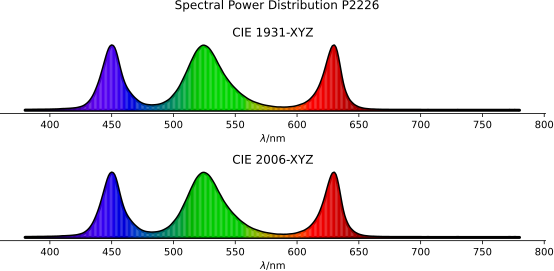
\includegraphics[width=0.65\textwidth]{./imgs/sec4/P2226-spd-n.pdf}
    \caption{P2226相对光谱分布图}
    \label{fig:P2226}
\end{figure}

P3030选用了GD\_DASPA2作为蓝色灯、GR\_DASPA2作为红色灯、GT\_DASPA2作为绿色灯。相对光谱分布(通道归一化)如图\ref{fig:P3030}所示。

\begin{figure}[htbp]
    \centering
    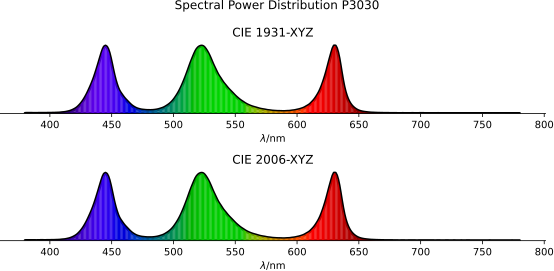
\includegraphics[width=0.65\textwidth]{./imgs/sec4/P3030-spd-n.pdf}
    \caption{P3030相对光谱分布图}
    \label{fig:P3030}
\end{figure}

由于P2226和P3030数据是以2nm为间隔的,为了方便统一处理,本文使用了三次样条插值进行处理,对部分光谱非固定间隔的进行了固定间隔化。结果如图\ref{fig:cmpdifled}所示。

\begin{figure}[htbp]
    \centering
    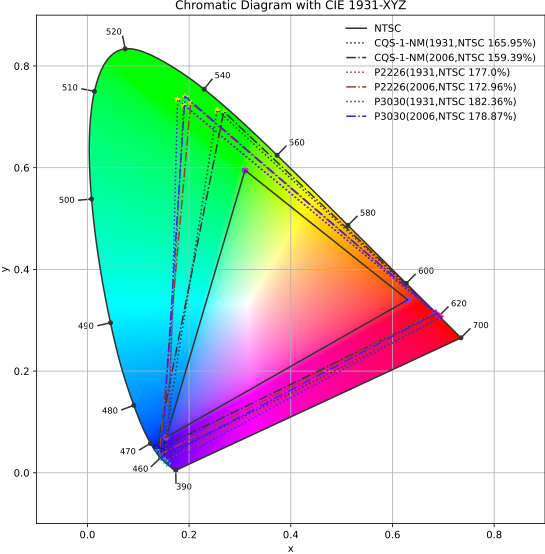
\includegraphics[width=0.65\textwidth]{./imgs/sec4/P3030-cmparea-sd.pdf}
    \caption{三种LED在两种色彩匹配函数中的色域对比}
    \label{fig:cmpdifled}
\end{figure}

从图中我们可以得知,两种色彩匹配函数表现的效果基本类似,圈定的范围重合度很高。从图上我们可以得到一个结论,3种LED的色域绿色都会向着左下角偏移(深绿),蓝色都会向着深蓝偏移(右下),红色基本不变,这是因为在2006版的色彩匹配函数中蓝色$\overline z$更集中了,导致蓝绿色在积分的时候Z值会更大,从而影响坐标,对R光而言较为远离影响不大。

从图中我们同时可以知道从1931转到2006,llab和P3030的LED的色域都减小了一点,P2226LED的色域反而增大了。我们观摩三个LED的相对光谱图\ref{fig:spd1931bgn},\ref{fig:P2226},\ref{fig:P3030}可以知道,llab和P3030相对于P2226来说更远离2006-XYZ的蓝色峰值,导致组成色域的蓝色点更接近其他两点,导致面积变小,色域定量范围变小,而P2226是更接近2006-XYZ蓝色峰值,因此色域变大,但影响都不大。总得来说这两种色彩匹配函数在实际应用中并没有很大的区别,只是蓝光处有些许影响。  % 总结
\section{色域最大化 -- 第四个基色}
从前面的色品图中我们可以看到RGB三色光所租成的色域,很明显的是,在此基础上再加上一个合适的单色光,必定会有更大的色域,由于时间不够,本文只对llab的数据进行探究,采用蓝色的光谱进行``位移'',视为新的单色光。本节以CIE 1931-XYZ色品图与色彩匹配函数作为探究前提。

\subsection{预搜寻--人工感知}

首先我们对色域三角形的三条边进行延拓,如图\ref{fig:sd1931-LINE}所示。

\begin{figure}[htbp]
    \centering
    \includegraphics[width=0.65\textwidth]{./imgs/sec5/CQS-1-NM-1931-Line.pdf}
    \caption{CIE 1931-XYZ色彩匹配函数下LED色域三角形延展}
    \label{fig:sd1931-LINE}
\end{figure}

从图上我们可以看到,左侧的空隙较大,若讨论单色光必定在460nm至530nm之间的单色光。即便讨论的不是单色光,直觉上第四个光源要使得色域最大化,应该要在蓝绿色分界线上,比如说靠近500$\sim$510nm的单色光的光谱直觉上会得到最大的色域。做研究不能只靠直觉,还得拥有数据,因此我们将在下一小节``复制平移''一个蓝色光源视为``第四色'',探究最大色域范围。

\subsection{程序搜寻--计算面积}

本小节的下的蓝光的中心波长为457nm,两个半功率点分别位于为451nm与463nm,因此我们最大蓝移为451nm$\rightarrow$380nm,最大红移为463nm$\rightarrow$780nm。蓝移部分有71个点,红移部分有317个点,将这些点绘制到色品图上,如图\ref{fig:sd1931-BLUEMOVE}所示。

\begin{figure}[htbp]
    \centering
    \includegraphics[width=0.65\textwidth]{./imgs/sec5/CQS-1-NM-4.pdf}
    \caption{蓝色LED平移}
    \label{fig:sd1931-BLUEMOVE}
\end{figure}

从图上我们可以得知,由于llab的LED数据较为纯净,平移后的结果比较靠近纯色光,在蓝移区基本贴近(需要放大看,这幅图有点吵眼睛)纯色光组成的马蹄边界。红移区需要到560nm后才基本贴近。由于第四个色出现的位置和面积计算有一些关联,比如说530nm$\sim$544nm的线段,若第四个色取自于这里,则得忽略绿色,进行新三角形的计算,而红色处在gr和rb交界上,蓝色也在bg和rb交界上,则可忽略这个问题,除了上面说的绿色特殊位置,都可以认为是一个四边形的计算,这些四边形和三角形的计算都可以由鞋带公式解决,以下部分操作部分由人工设置,非完全自适应。后续操作流程如下所示。
\begin{itemize}
    \item [1. ]计算特殊区域三角区,得到该三角区范围为534$\sim$542nm(平移后的中心),详细请见{\bf scripts/plot\_sd4\_findP.py}文件。
    \item [2. ]根据区域分段计算面积(采用鞋带公式计算三角形与四边形的面积),然后保存在一个数组中
    \item [3. ]寻找这个数组中的最大元素,找到对应的xy
    \item [4. ]根据xy值转到xyY系统再转XYZ系统再转sRGB得到对应颜色
    \item [5. ]画出该光功率谱,并查阅相关资料获取该RGB值的颜色名称
\end{itemize}
以上计算的完成为穷尽法,详情请见文件{\bf scripts/plot\_sd4\_final.py}。我们发现,红移51nm后得到以508nm为中心的光的面积最大,为0.24164,RGB值为\#00FF6B(归入0$\sim$255后取四舍五入),即$(r,g,b)=(0,255,107)$也符合我们前面的直觉。该颜色的光谱图\ref{fig:spd1931-color4}如所示。

\begin{figure}[htbp]
    \centering
    \includegraphics[width=0.65\textwidth]{./imgs/sec5/CQS-1-NM-spd-4.png}
    \caption{第四光源的光谱图(CIE 1931-XYZ)}
    \label{fig:spd1931-color4}
\end{figure}


处理后得到的最大面积色域与色品图如图所示\ref{fig:spd1931-4final}所示。

\begin{figure}[htbp]
    \centering
    \includegraphics[width=0.65\textwidth]{./imgs/sec5/CQS-1-NM-4-final.pdf}
    \caption{第四光源的光谱图(CIE 1931-XYZ)}
    \label{fig:spd1931-4final}
\end{figure}

\subsection{结论}
我们从上面了解到该颜色光的RGB为$(r,g,b)=(0,255,107)$,换为16进制为\#00FF6B,这种颜色的名字没有确切定义\footnote{https://www.htmlcsscolor.com/hex/00FF6B},类似于春绿色(Spring Green,\#00FF7F),本文暂称其为类春绿色。我们认为加上类春绿色的光源将会令llab数据的色域范围最大。由于时间问题,本文不讨论P2226与P3030的情况。由于该部分完成的较为急迫,代码相对繁杂且冗余过多。

  % 应用
\section{总结}

由于自身并非做光学相关的领域,研究领域也与光没有很直接的联系,对光学的了解甚微,出于好奇选择了这门课。光学基础薄弱一时间难以明白前几个题目的思路,因此选择这个不需要过多的光学知识与背景的题目作为期末作业。

本题目的四个子目标本文都基本完成,对有了色度学更深的认知与理解,明白了成色的原理以及一些色度的概念与定义,在第三个子目标中分析较为欠缺,第四个子目标中完成度较低,设置较为粗糙。总体来说达到了自身满意的水平,毕竟在开始做的时候只知道RGB与存在混色原理,对其他东西一窍不通,最后做出了一个差强人意的结果,感觉已经达到预期水准。最后吐槽以下,RGB三基色LED灯珠的数据真的太难找了,本次作业的一半的有效工作时间都在找数据与找数据的路上,由于相关知识的欠缺与渠道的阻塞,费劲千辛万苦才找到了原始数据,虽然不清楚其是否标准,但起码比从图像中扣要合理,曾几何时我想过从论文中的QLED图扣下来,后面也因为找到勉强能用的数据才就此罢休。本文主要使用了宾夕法尼亚州立大学llab的数据,也从中获取到了很多xyz计算的思路。本文中部分图是jupyter(ipynb)中保存的,可能py后缀的文件中没有直接对应的功能,需要部分的修改才能重新。

本次大作业让我学会了很多的色度学知识,虽然这些知识对我未来的研究学习可能并没有很明显的帮助,但是本次大作业拓展了我对色度、色域相关的认知,对我日后生活有较大的帮助,因为可以更懂得如何评价一个显示器、设备的好坏,不易买到不合适的产品。最后,感谢老师们的教导,让我对光学了解更多了。虽然由于前置知识的欠缺大部分内容听不太懂,但也增广了见识。  % 总结
\endgroup

\medskip
{\small{}\bibliographystyle{./reference/gbt7714-2005.bst}
\bibliography{./reference/report}
}{\small\par}

\end{document}